\documentclass[a4paper]{article}

%% Language and font encodings
\usepackage[english]{babel}
\usepackage[utf8x]{inputenc}
\usepackage[T1]{fontenc}
\usepackage{amsmath}

%% Sets page size and margins
\usepackage[a4paper,top=3cm,bottom=2cm,left=3cm,right=3cm,marginparwidth=1.75cm]{geometry}

%% Useful packages
\usepackage{amsmath}
\usepackage{graphicx}
\usepackage[colorinlistoftodos]{todonotes}
\usepackage[colorlinks=true, allcolors=blue]{hyperref}

\title{Cheatsheet for Fisher-Rao Metric, Geometry, and Complexity of Neural Networks}
\author{Sandro Braun, Leander Kurscheidt}

\begin{document}
\maketitle
\begin{abstract}
\end{abstract}
\section{Geometry of Deep Rectified Networks}

Lemma 2.1 (Structure in Gradient)
\begin{align}
	\sum_{t=0}^{L} \sum_{i \in [k_t], j \in [k_{t+1}]} \frac{\partial O^{L+1}}{\partial W^{t_{ij}}} W^t_{ij} = (L+1)O^{L+1}(x) = \langle \nabla_\theta f_\theta (x), \theta \rangle
\end{align}

\begin{figure}
	\centering
	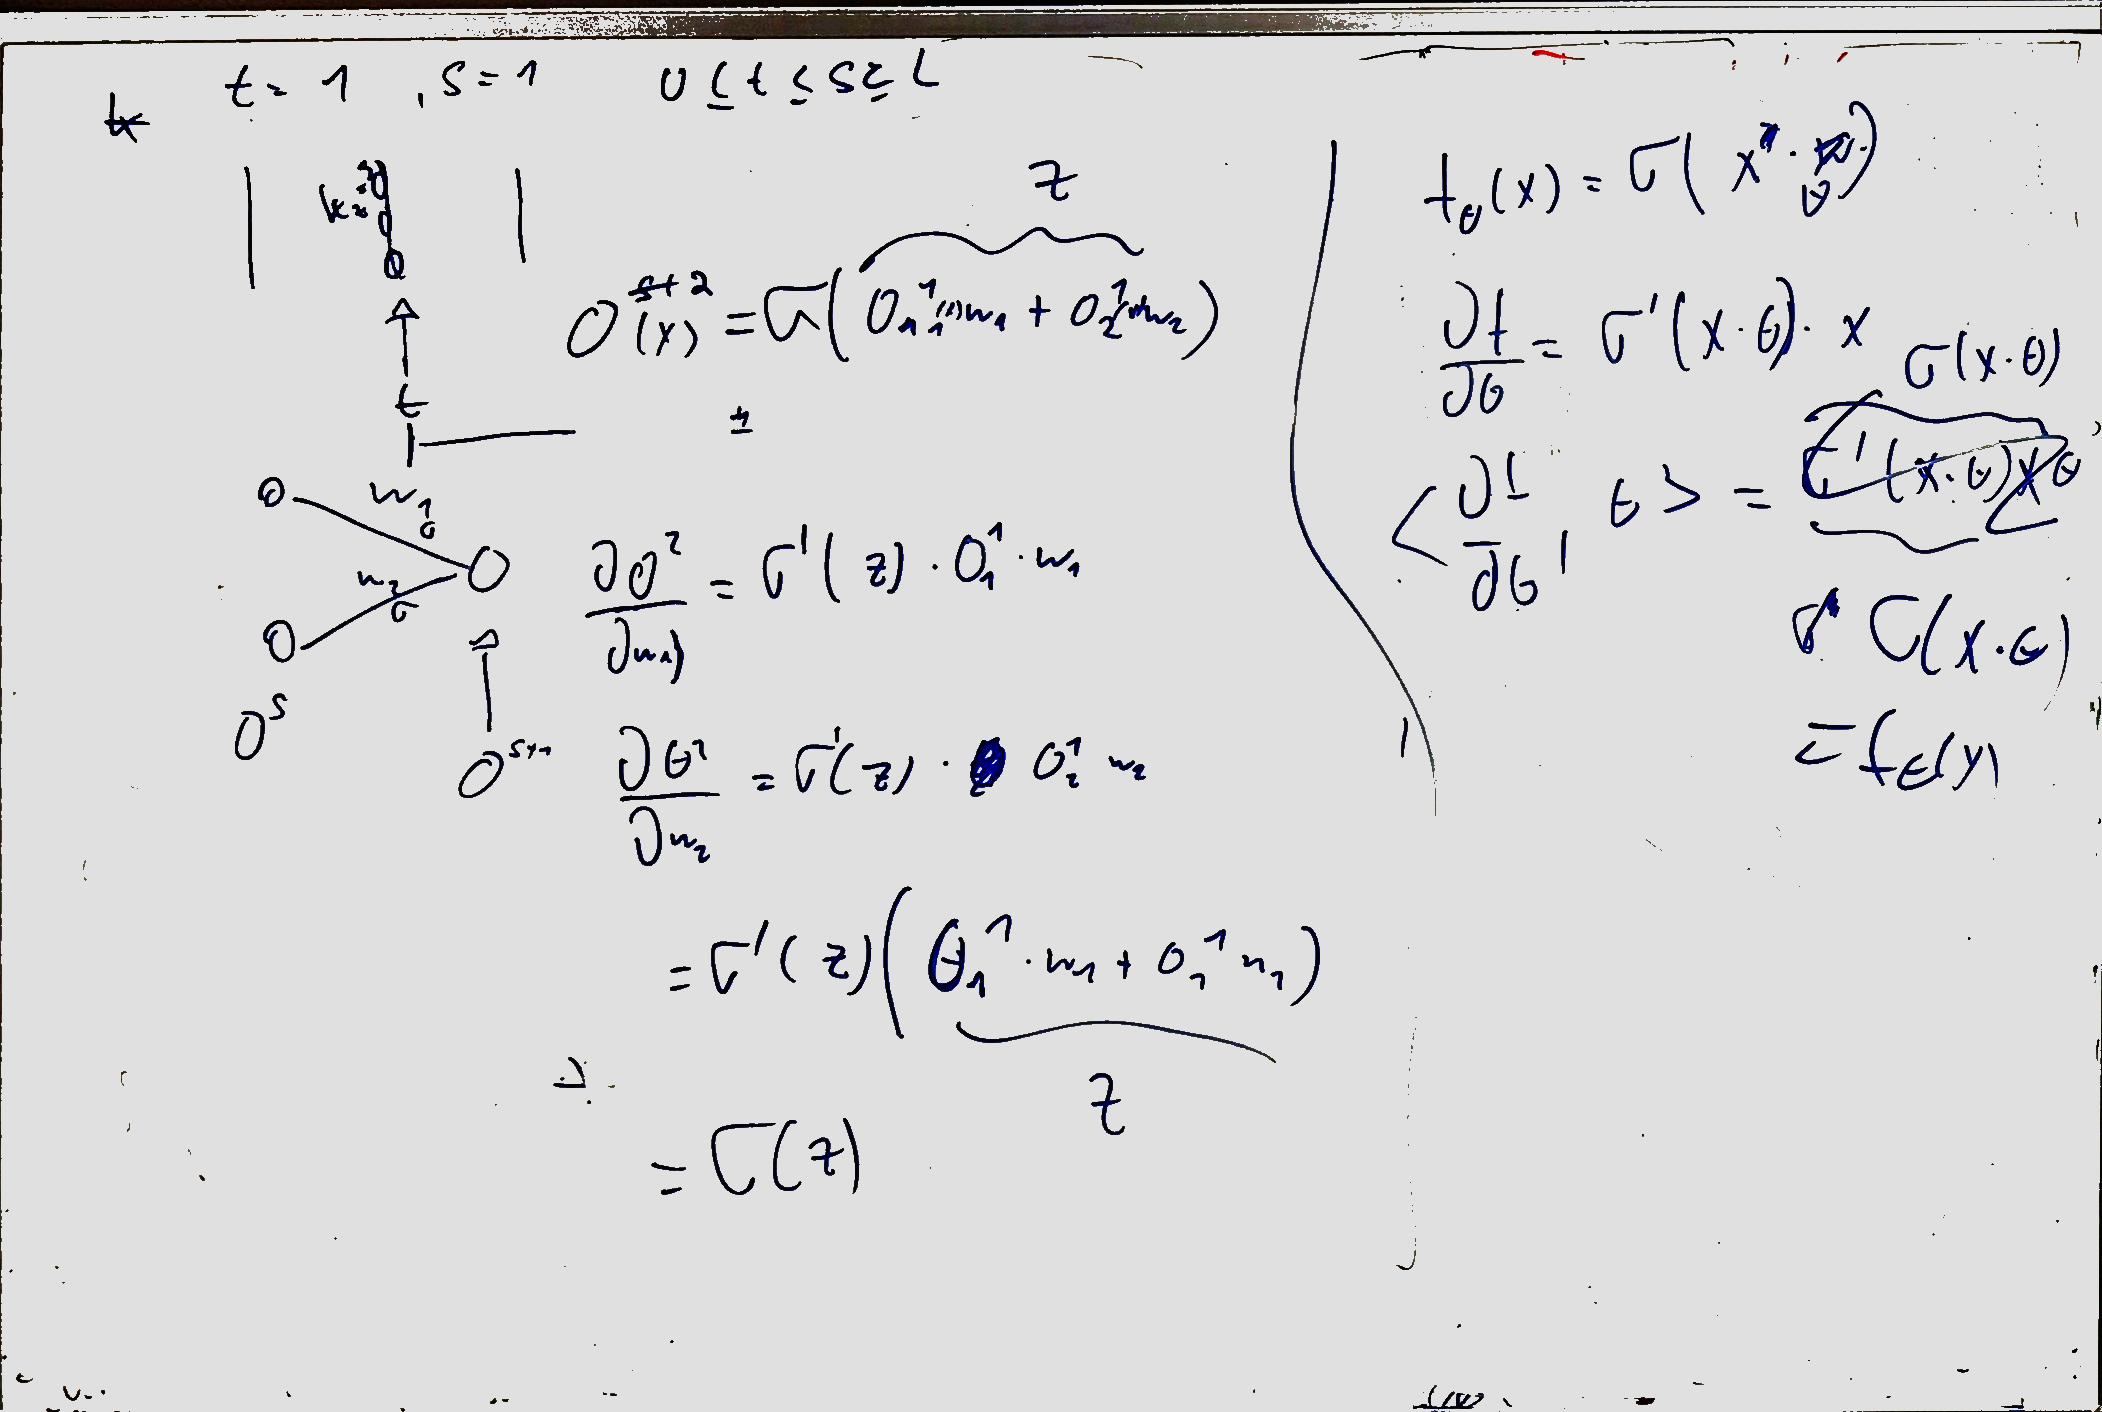
\includegraphics[width=\textwidth]{whiteboard_notes/20180706_01.jpg}
\end{figure}

\begin{figure}
	\centering
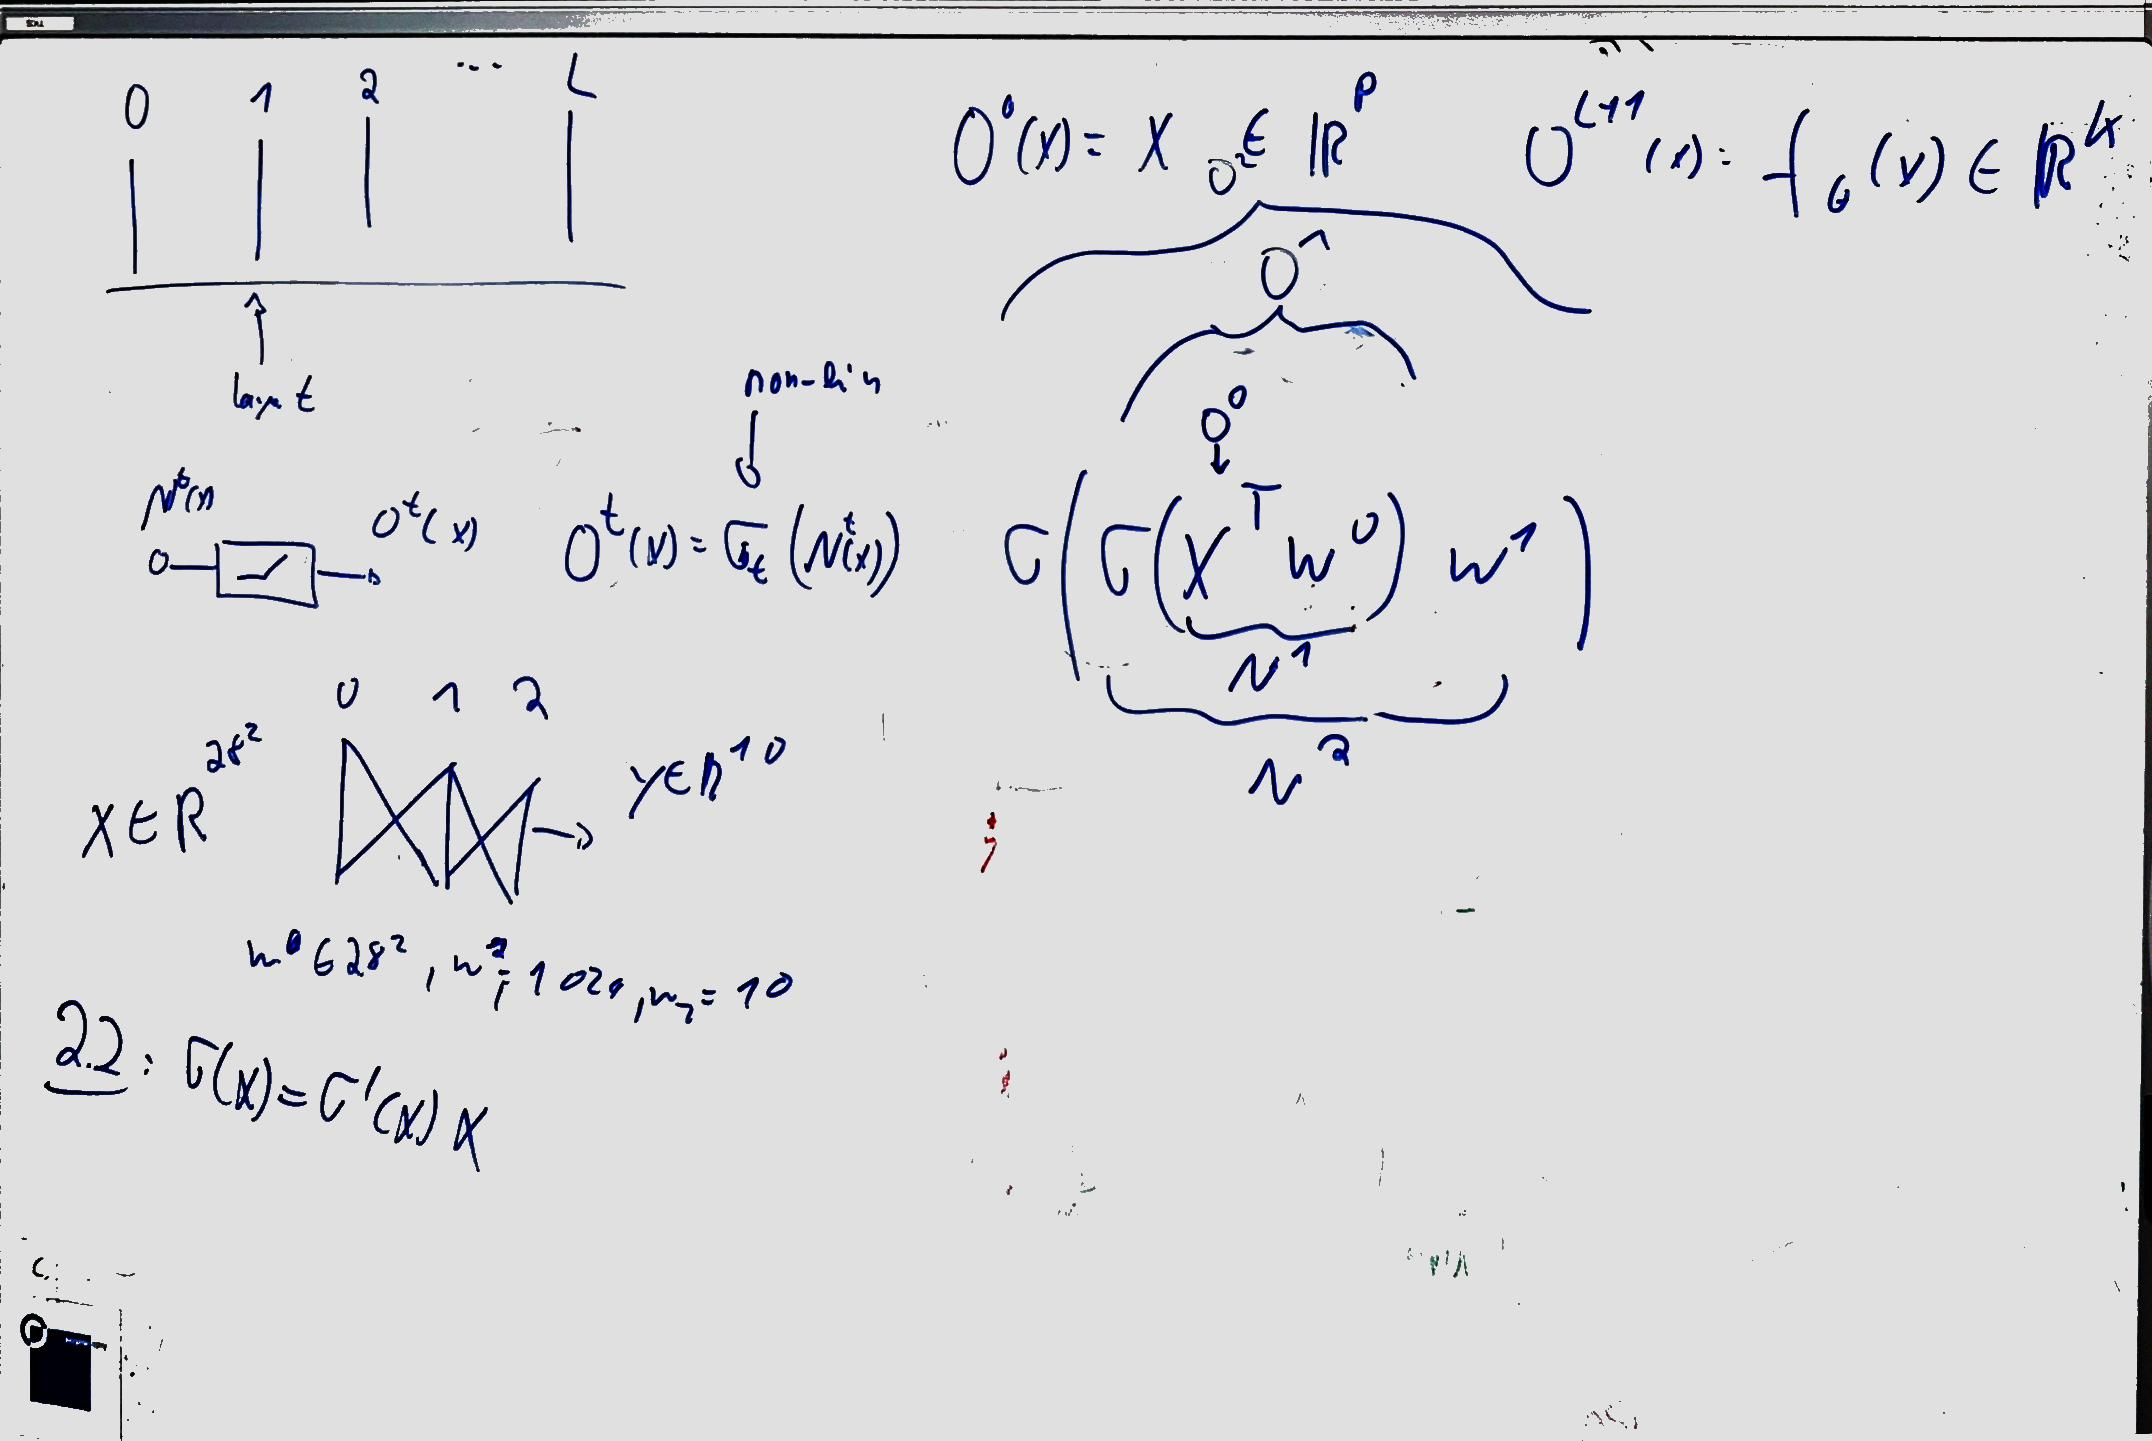
\includegraphics[width=\textwidth]{whiteboard_notes/20180706_02.jpg}
\end{figure}
\begin{figure}
	\centering
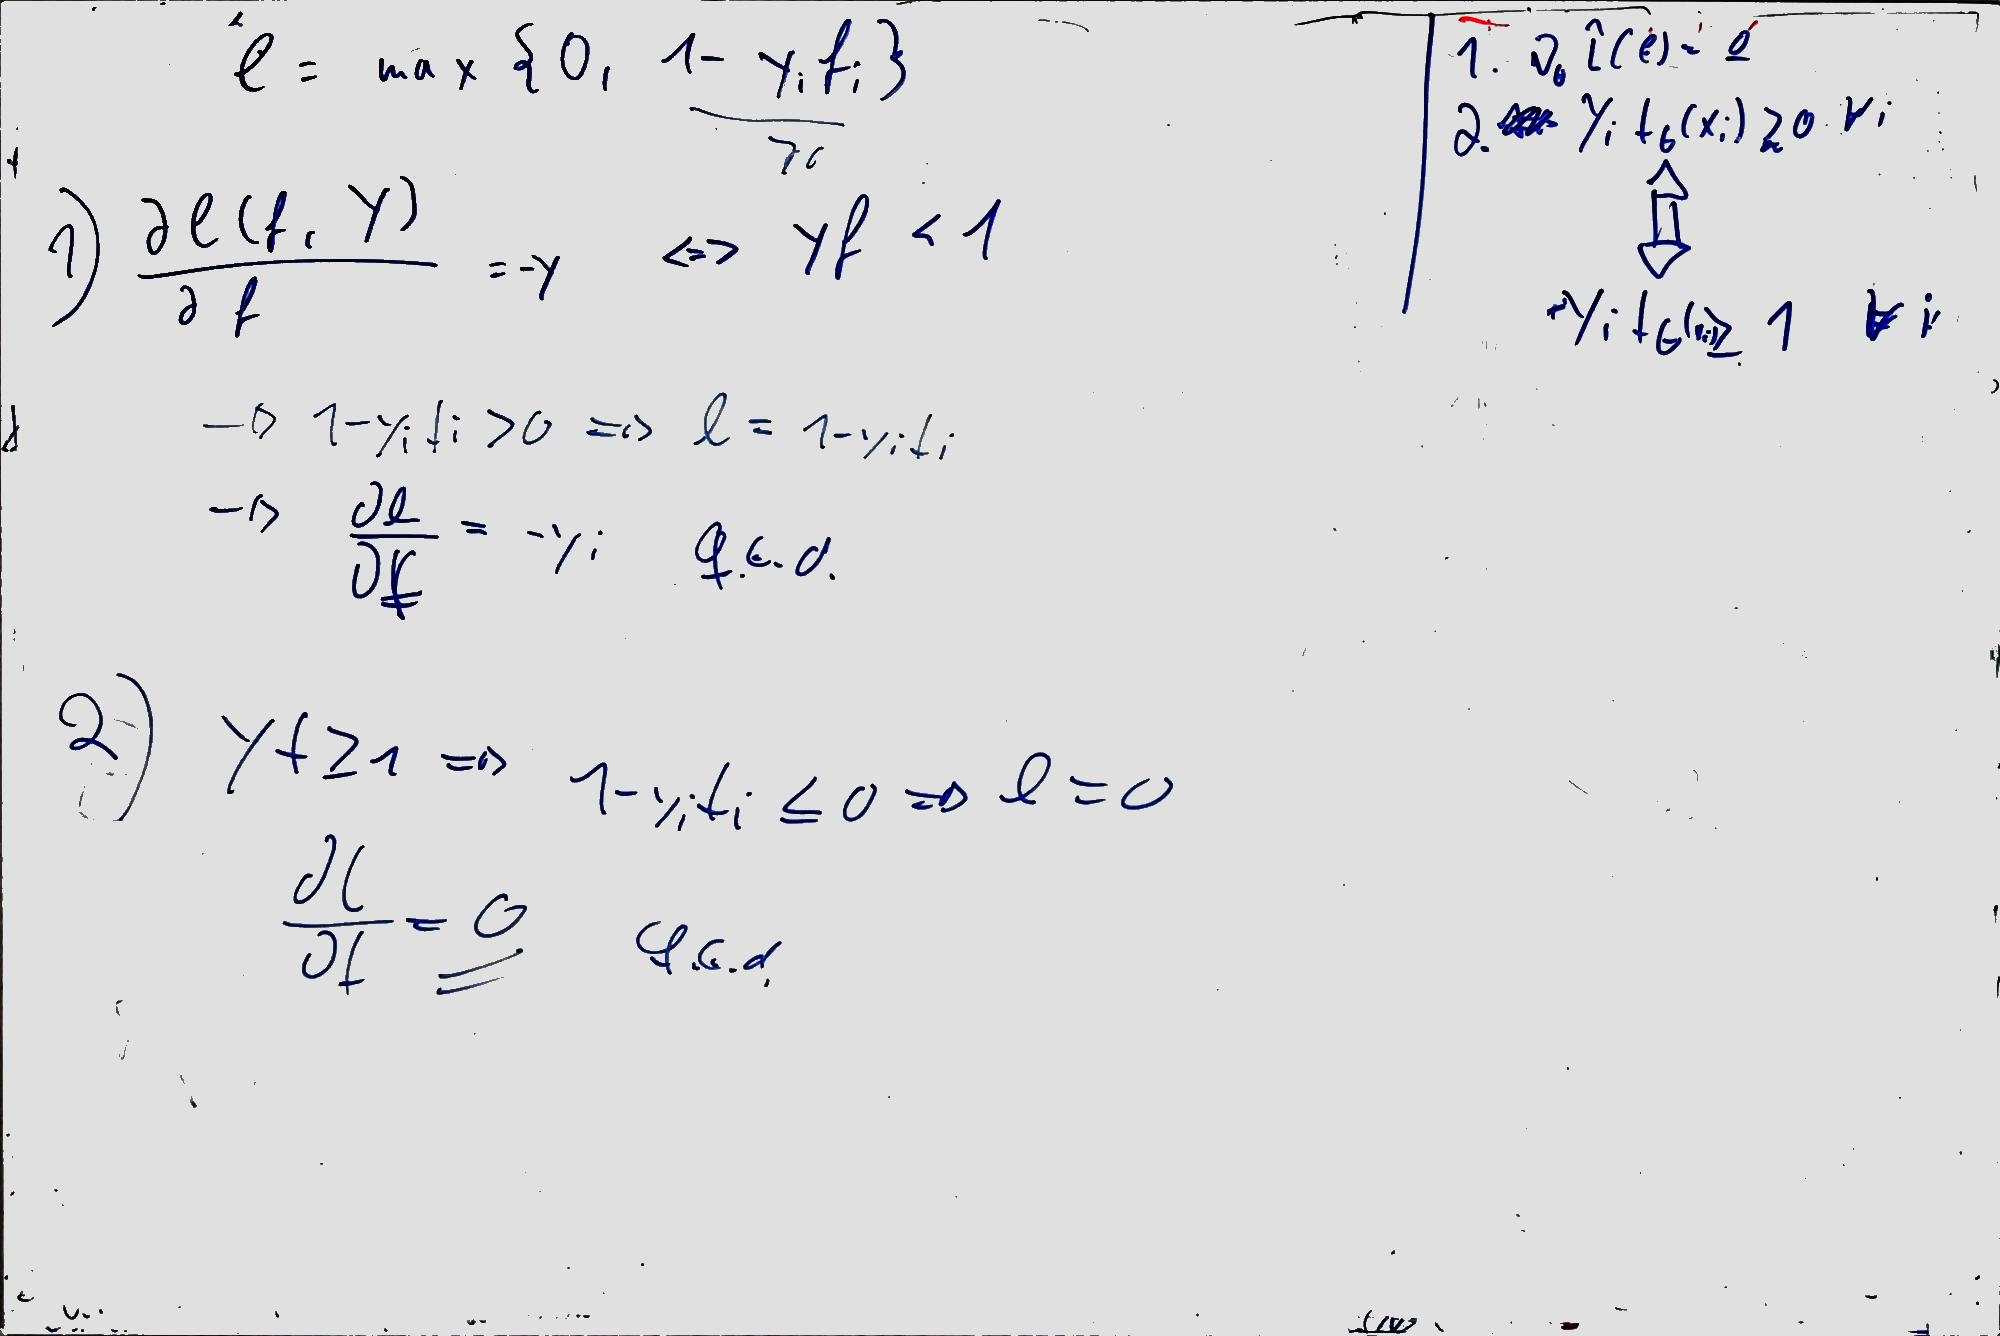
\includegraphics[width=\textwidth]{whiteboard_notes/20180706_03.jpg}
\end{figure}
\begin{figure}
	\centering
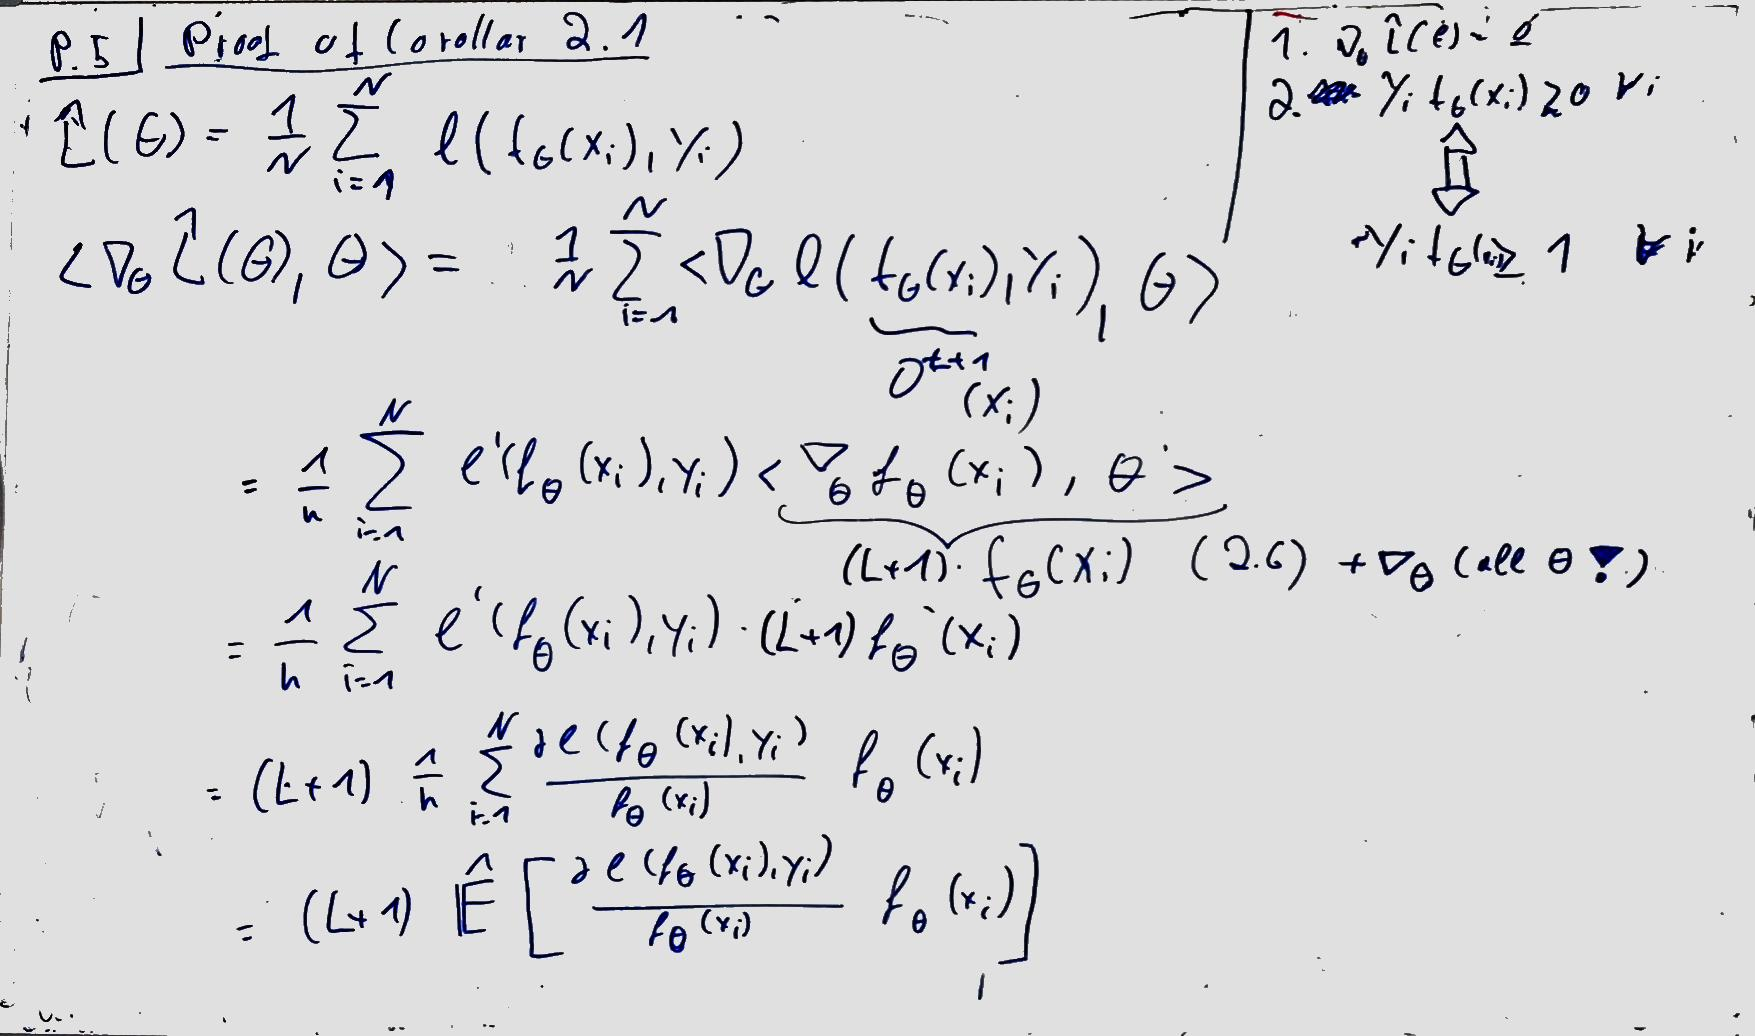
\includegraphics[width=\textwidth]{whiteboard_notes/20180706_04.jpg}
\end{figure}
\begin{figure}
	\centering
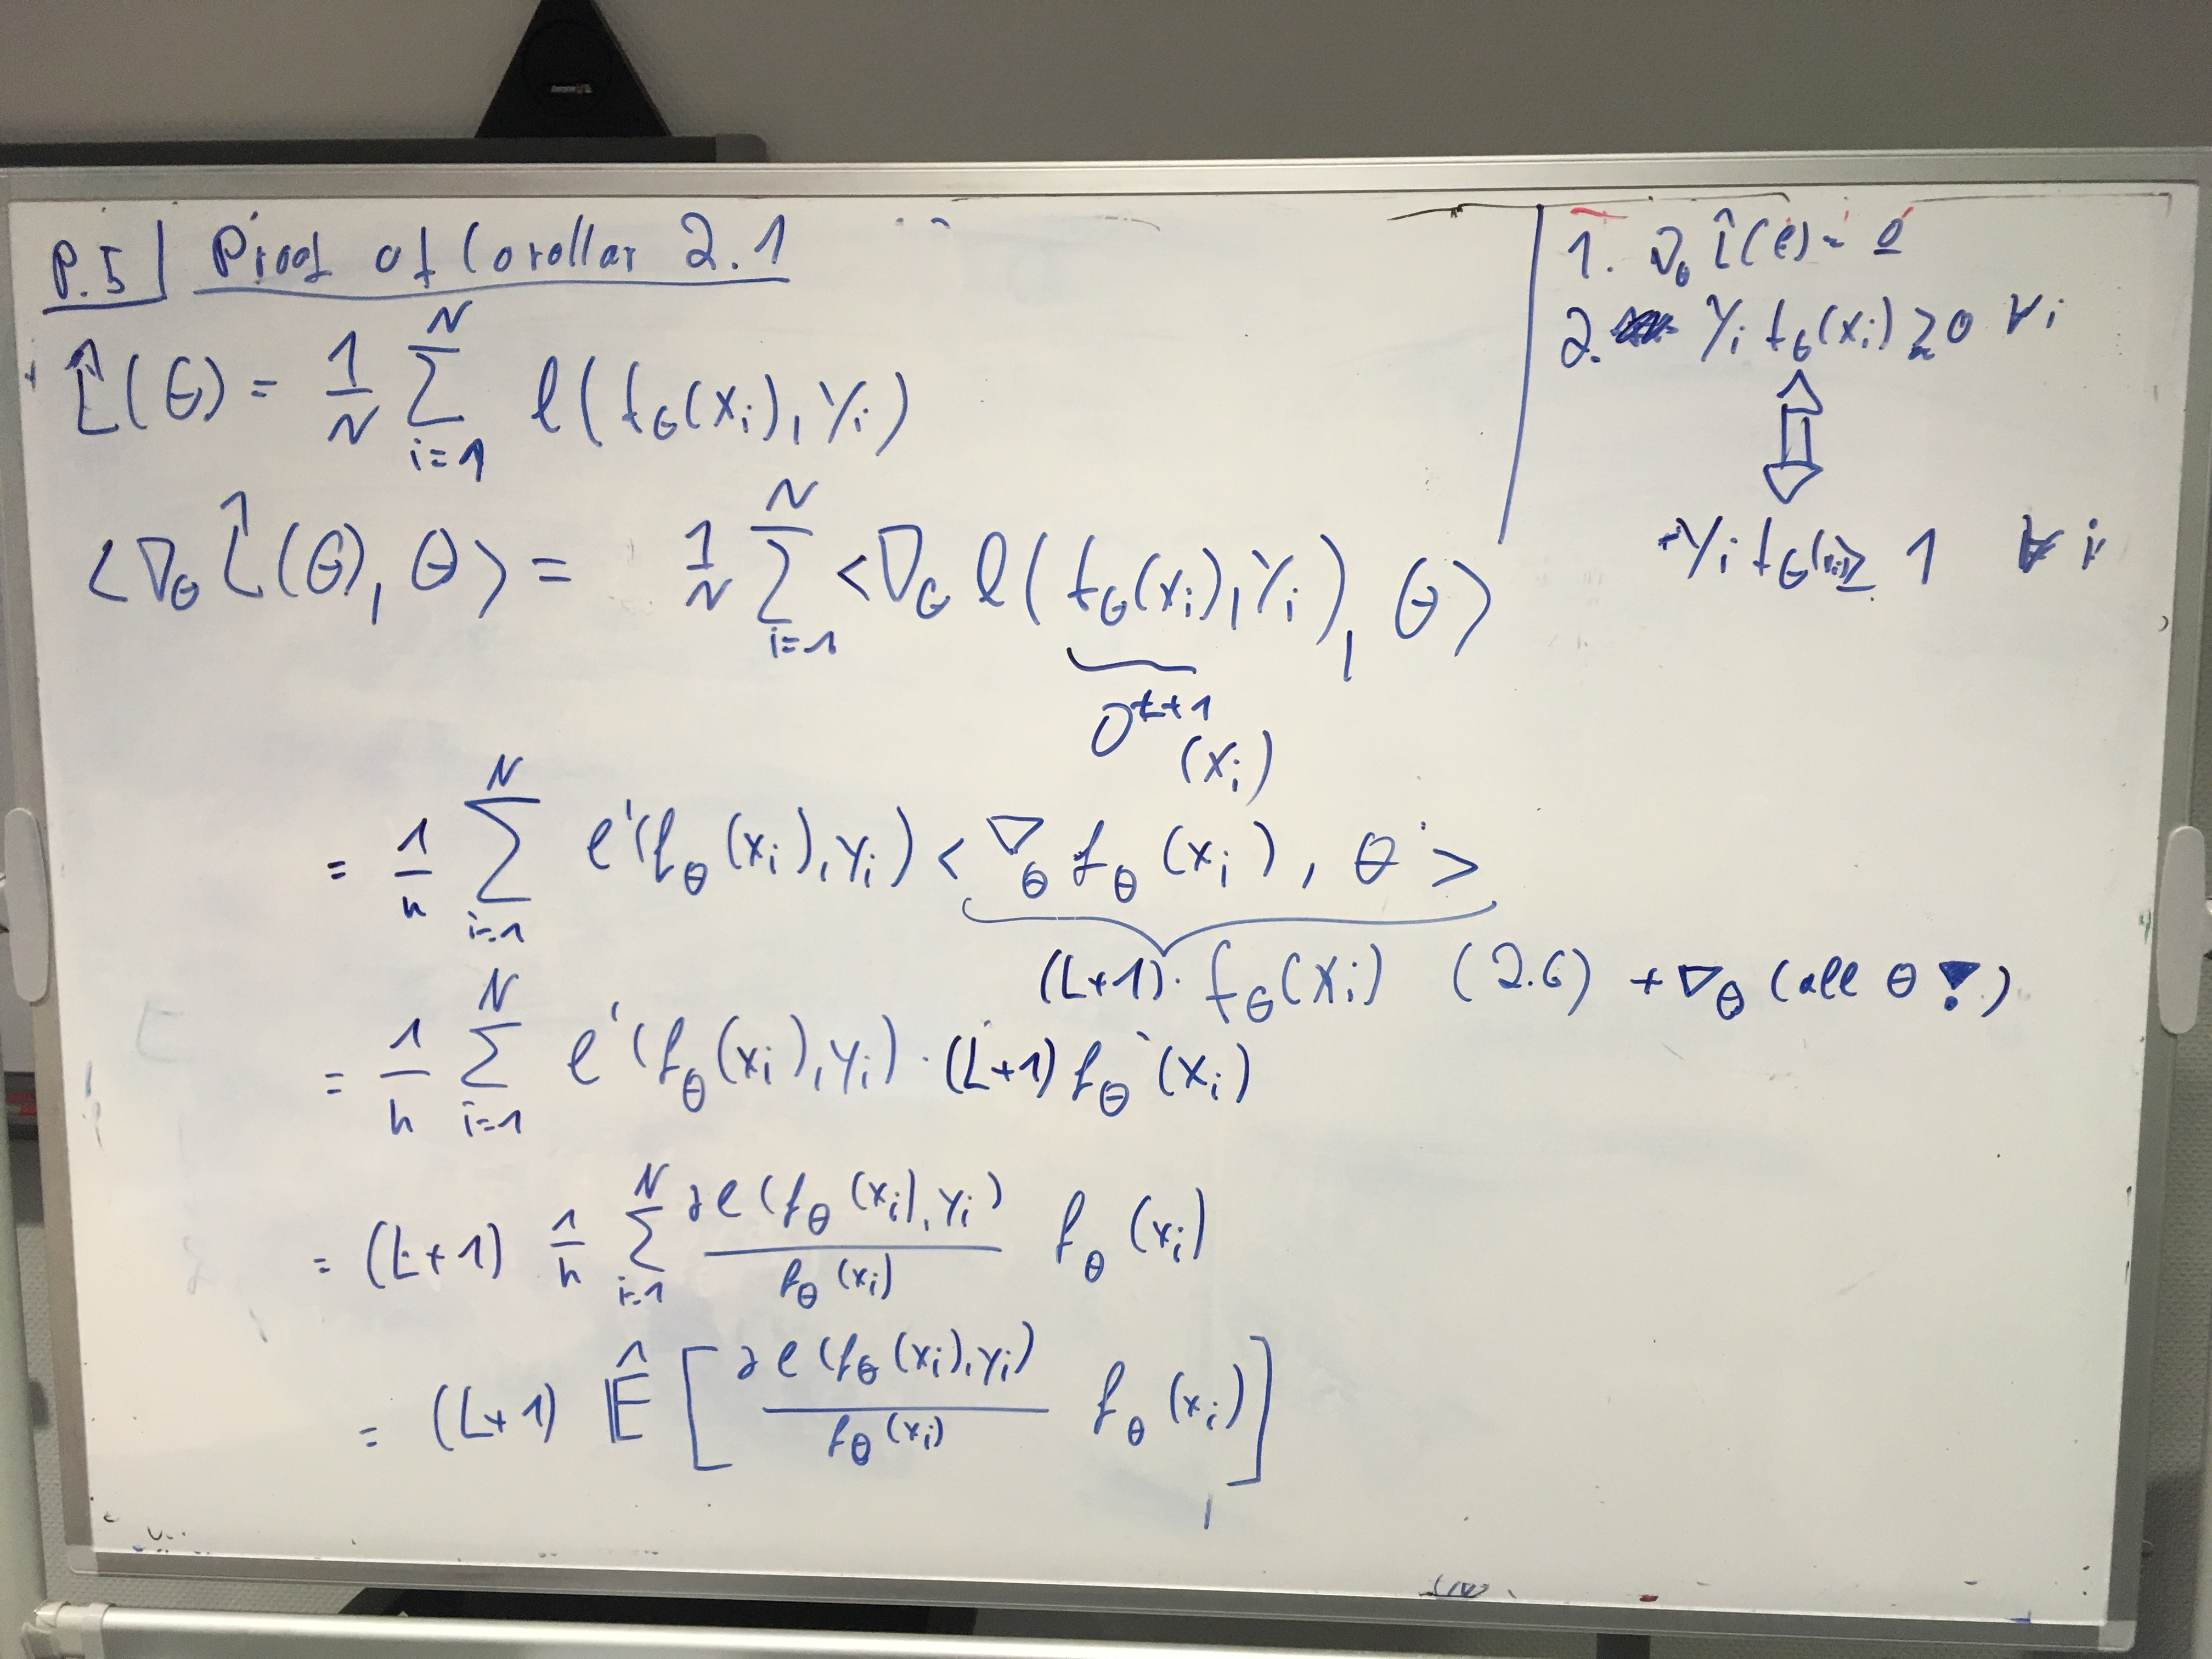
\includegraphics[width=\textwidth]{whiteboard_notes/IMG_1583.jpg}
\end{figure}
\begin{figure}
	\centering
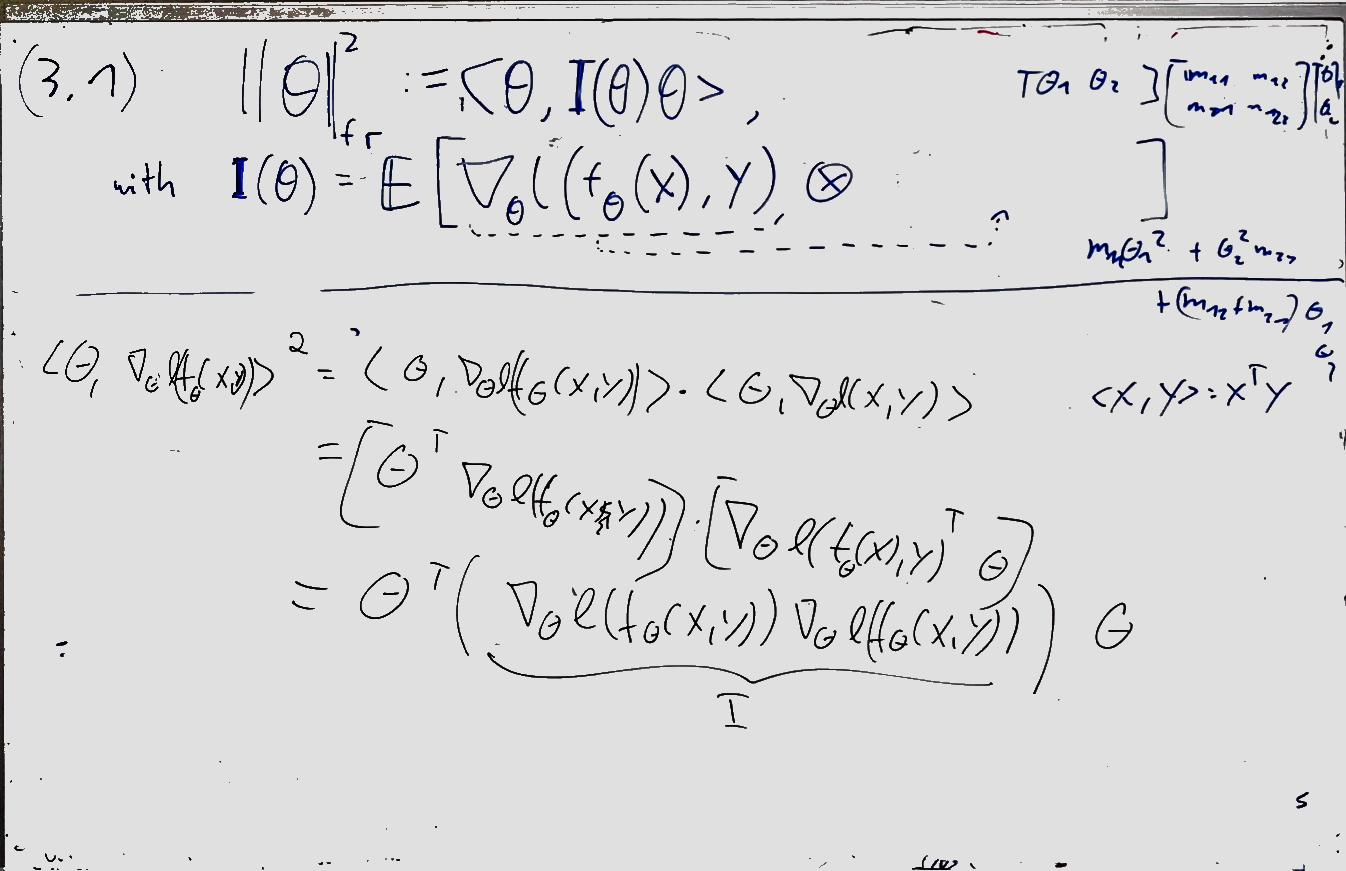
\includegraphics[width=\textwidth]{whiteboard_notes/3_1_proof.jpg}
\end{figure}
\begin{figure}
	\centering
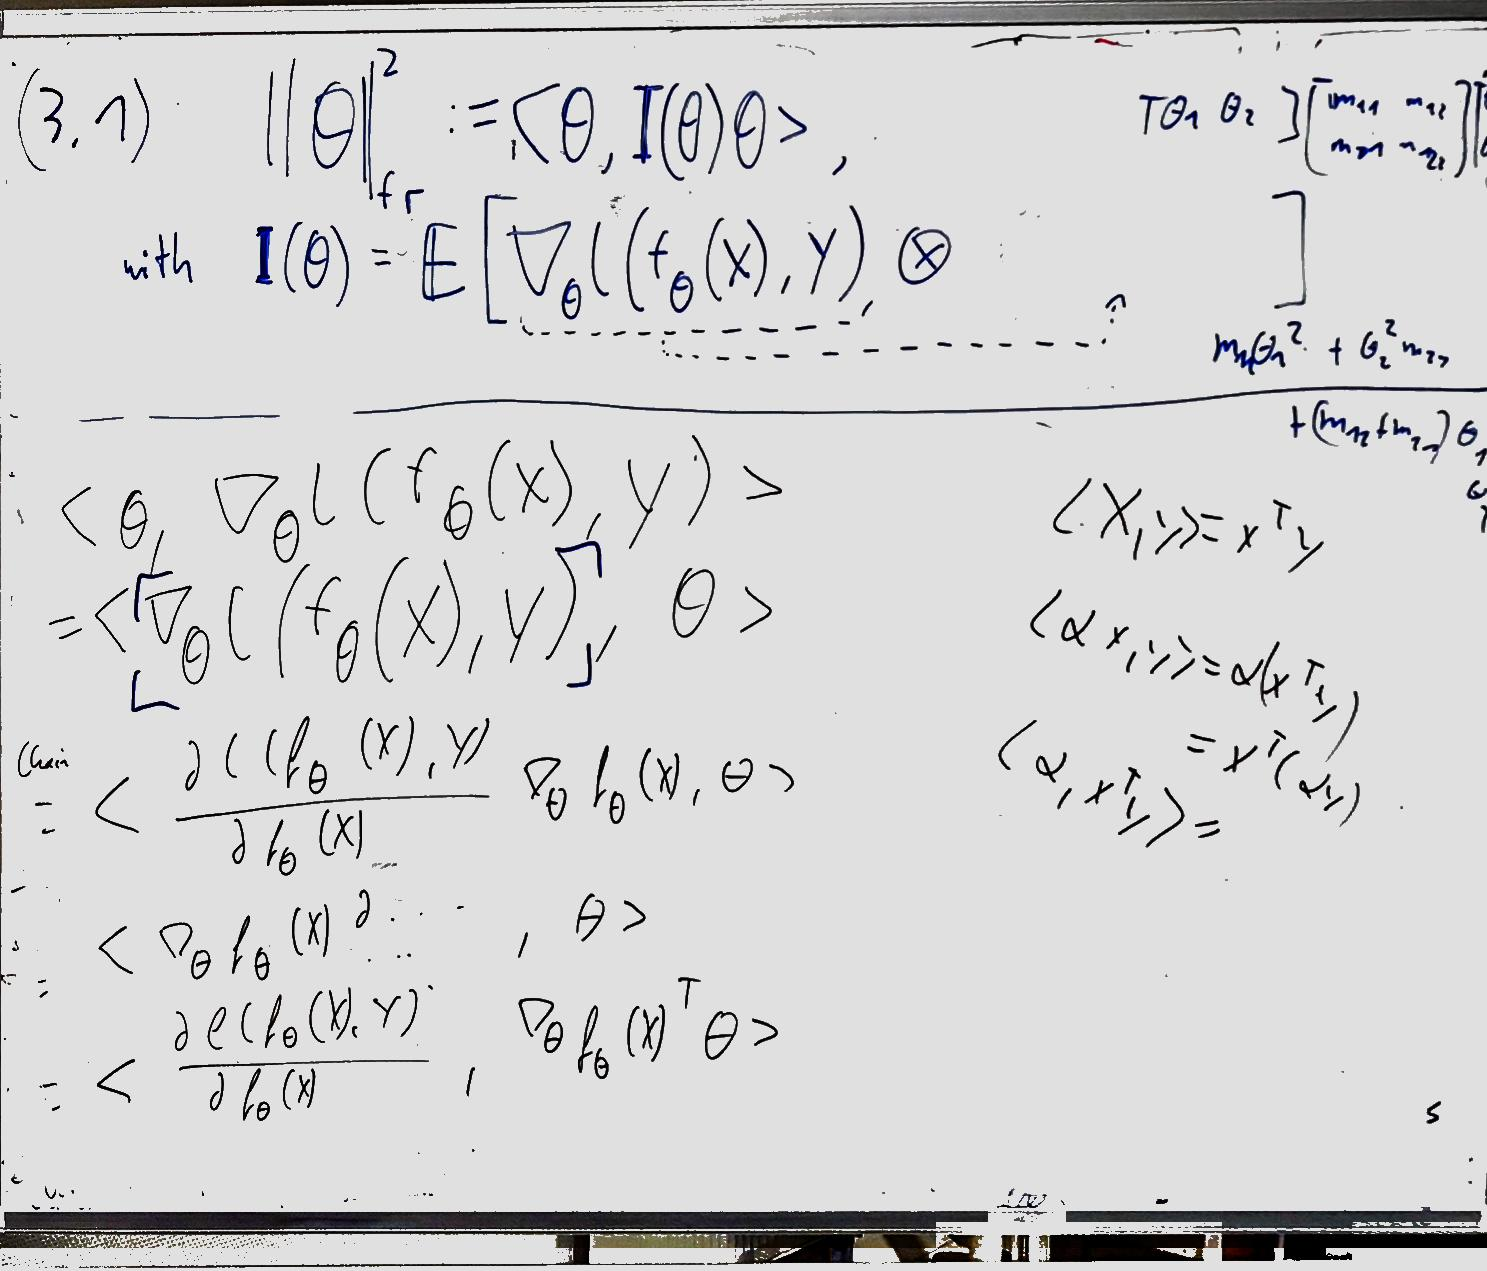
\includegraphics[width=\textwidth]{whiteboard_notes/3_1_proof_cont.jpg}
\end{figure}
\begin{figure}
	\centering
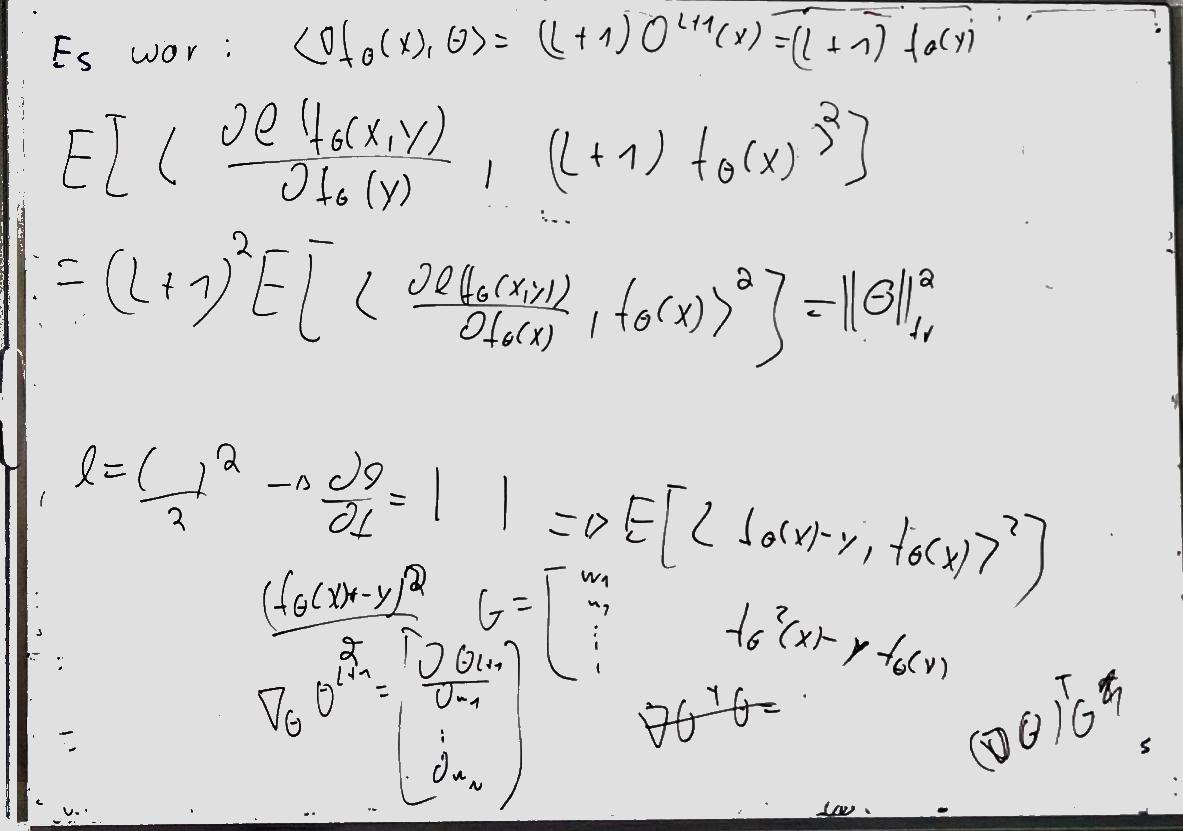
\includegraphics[width=\textwidth]{whiteboard_notes/07.jpg}
\end{figure}
\begin{figure}
	\centering
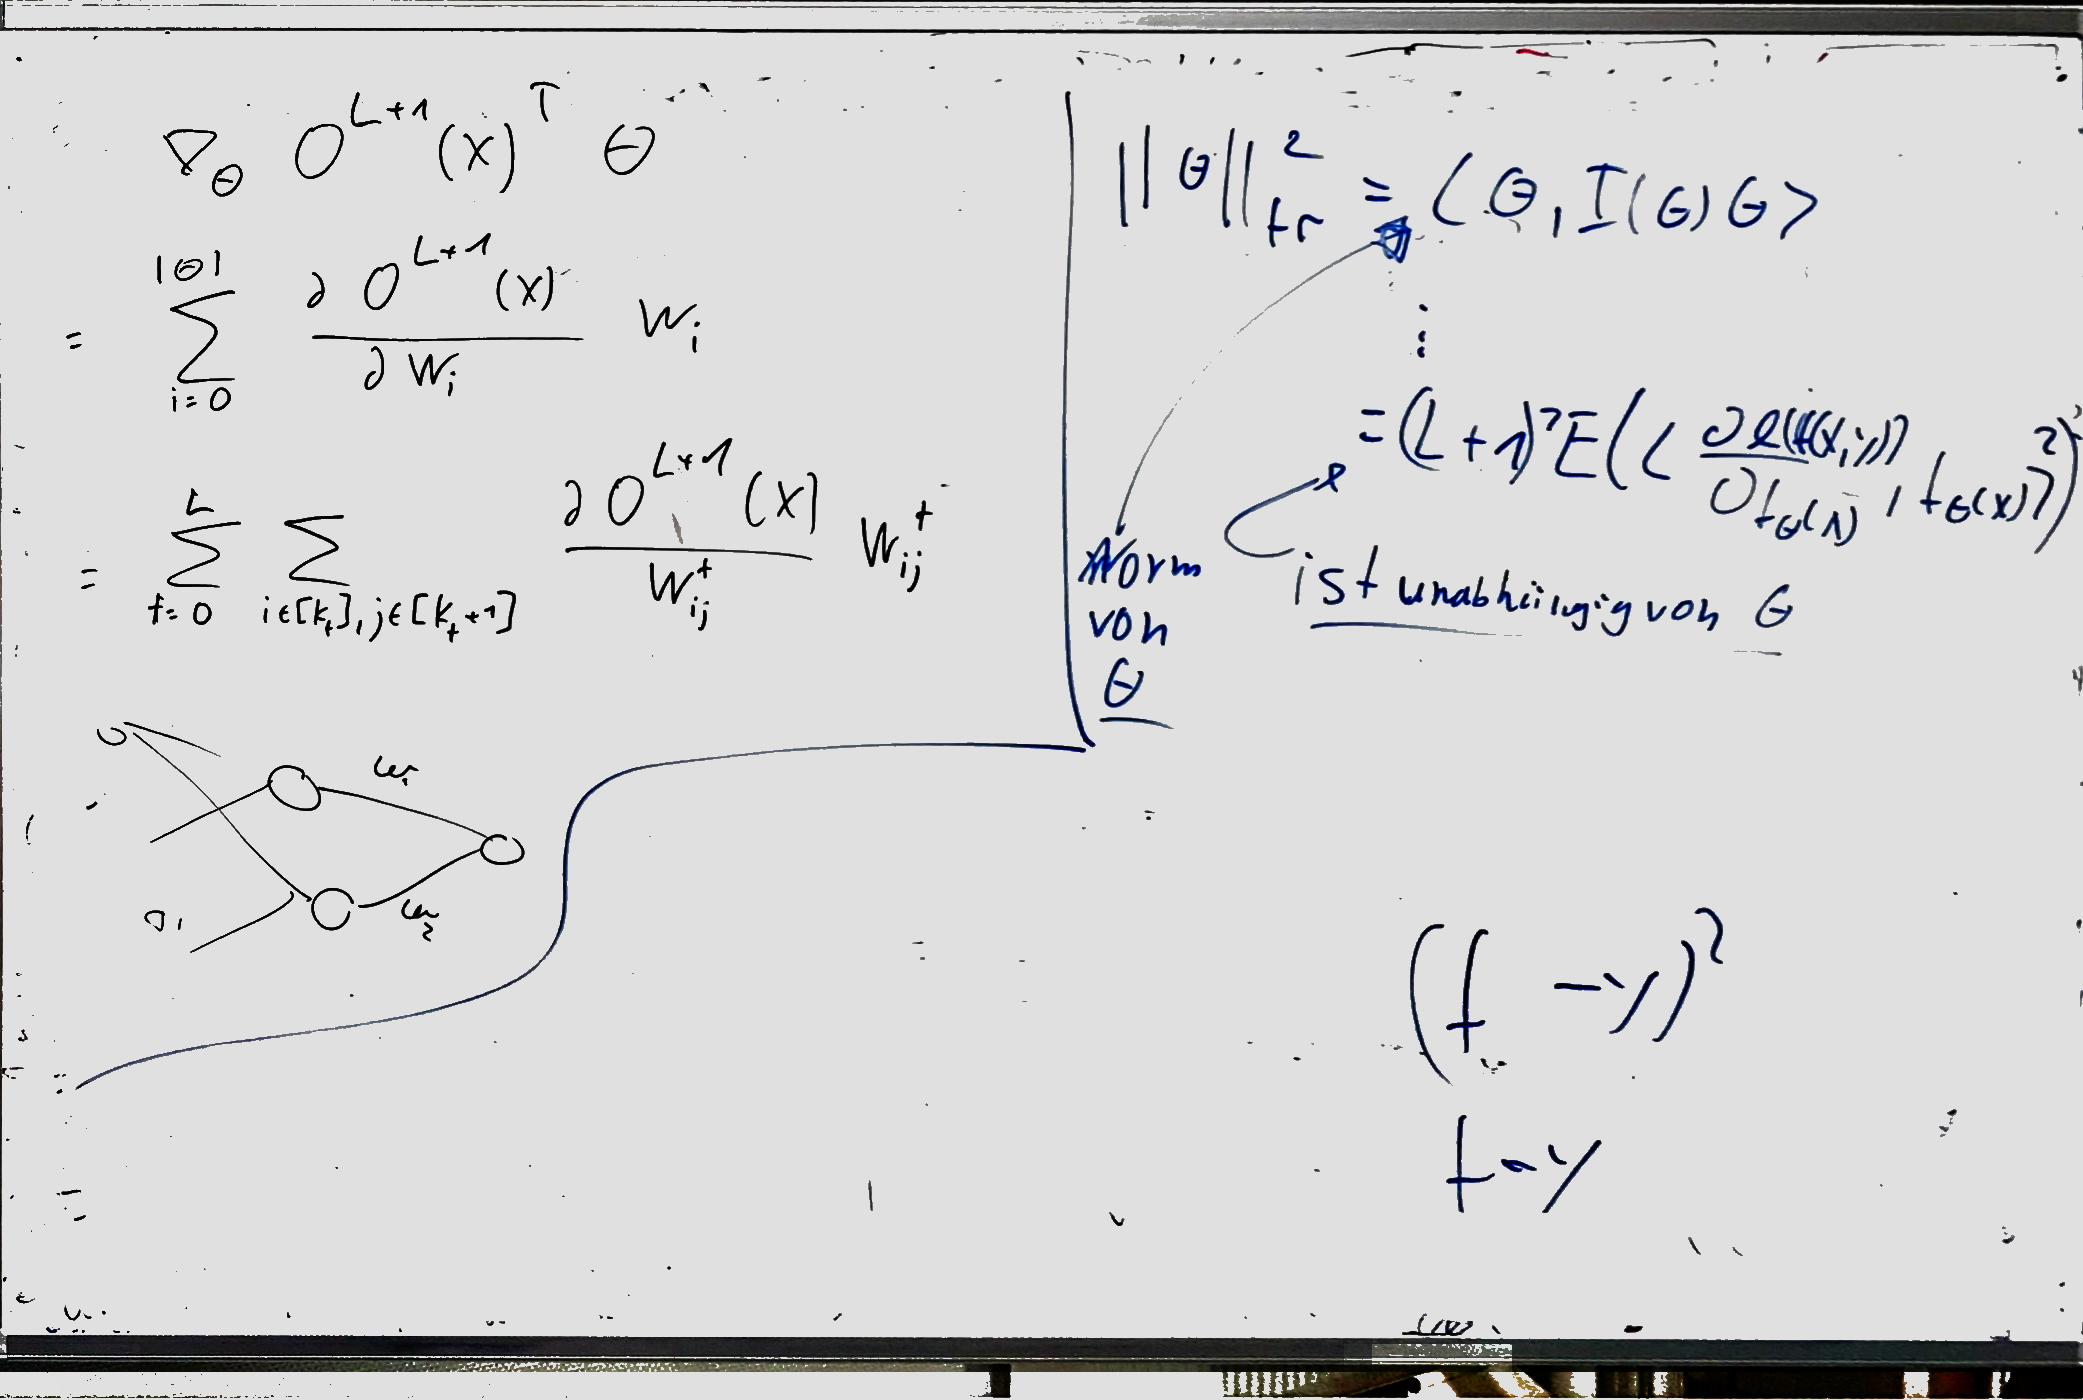
\includegraphics[width=\textwidth]{whiteboard_notes/08.jpg}
\end{figure}

\begin{figure}
	\centering
	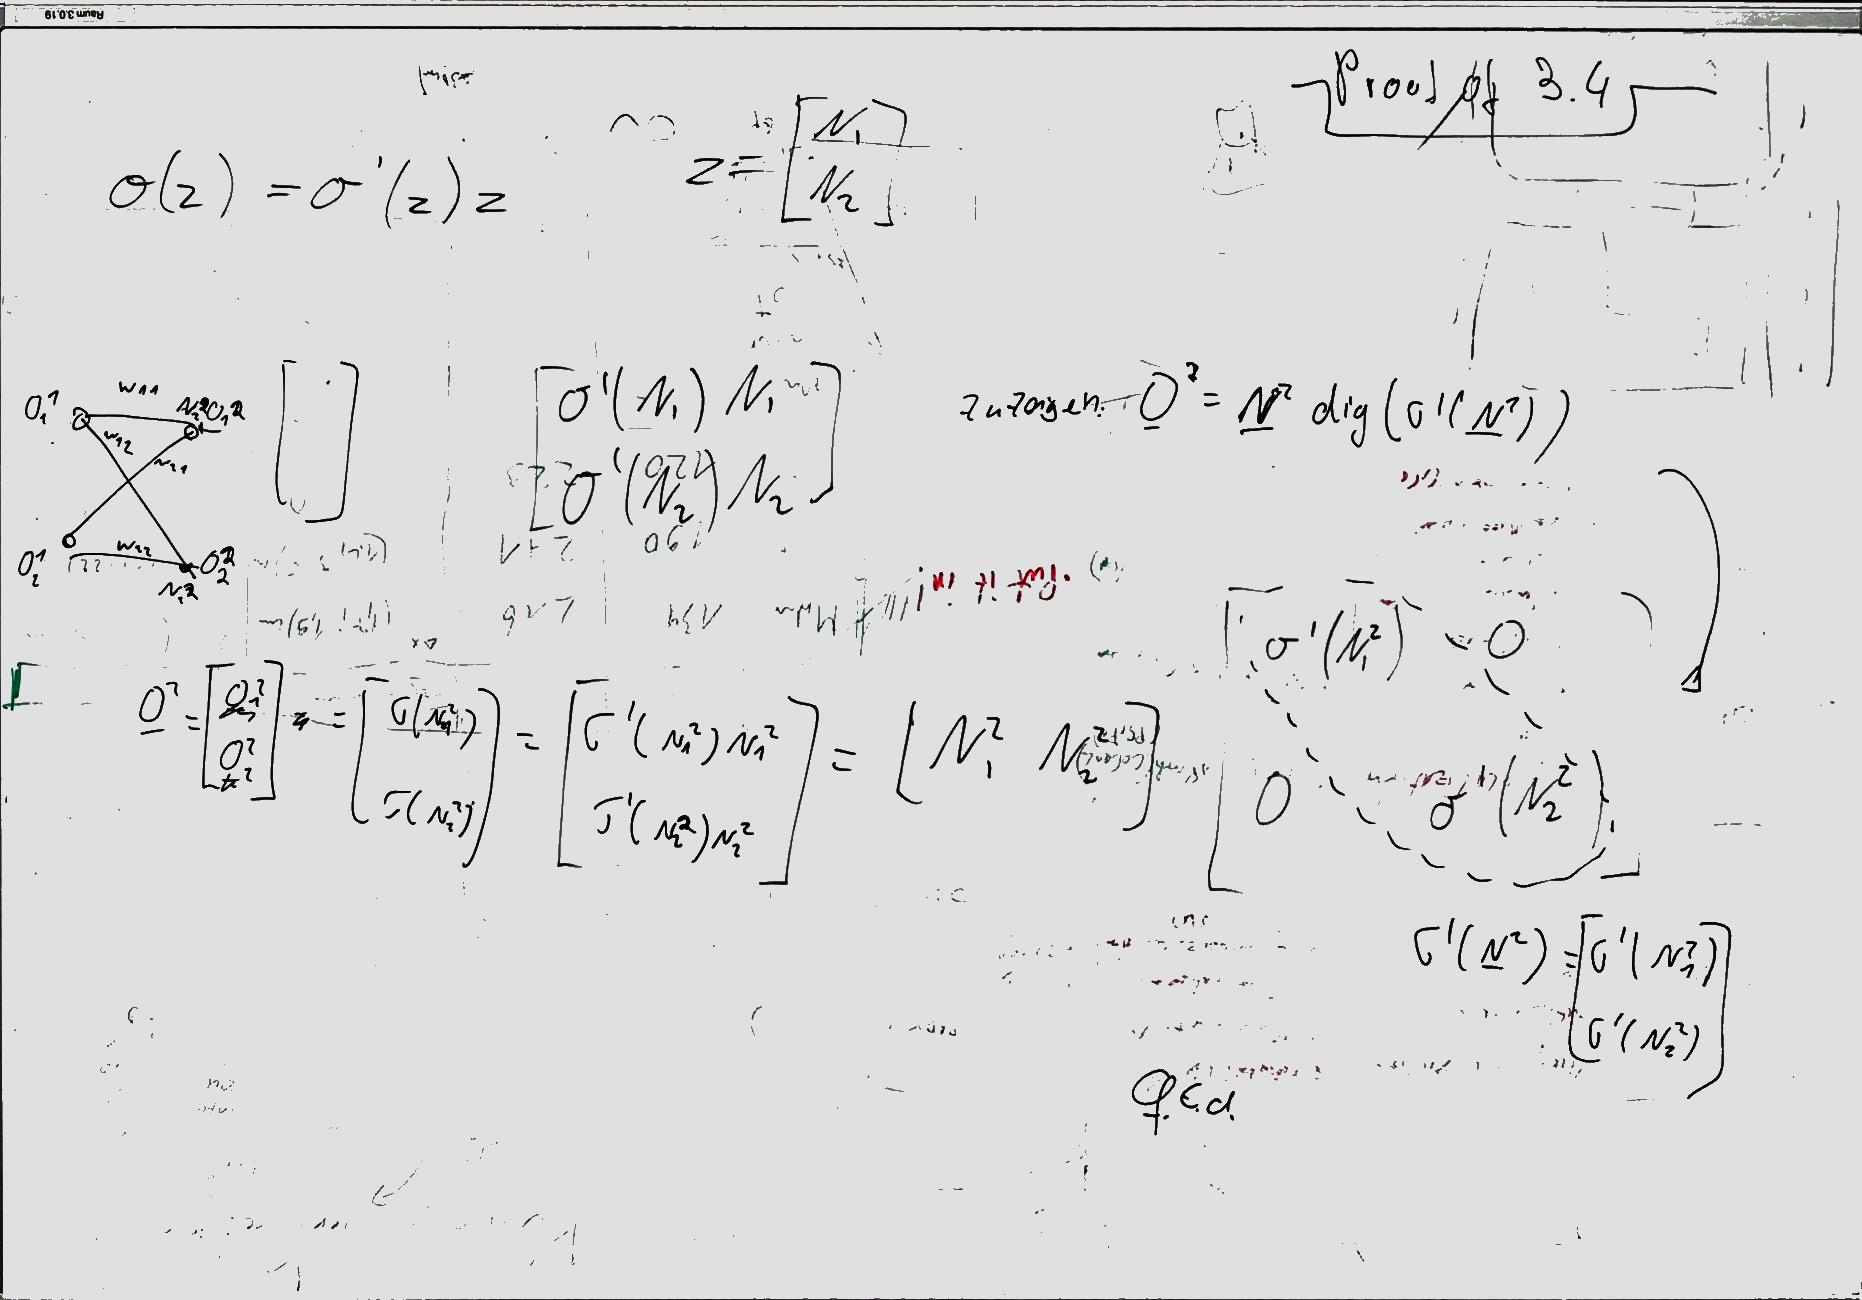
\includegraphics[width=\textwidth]{whiteboard_notes/09.jpg}
\end{figure}

\begin{figure}
	\centering
	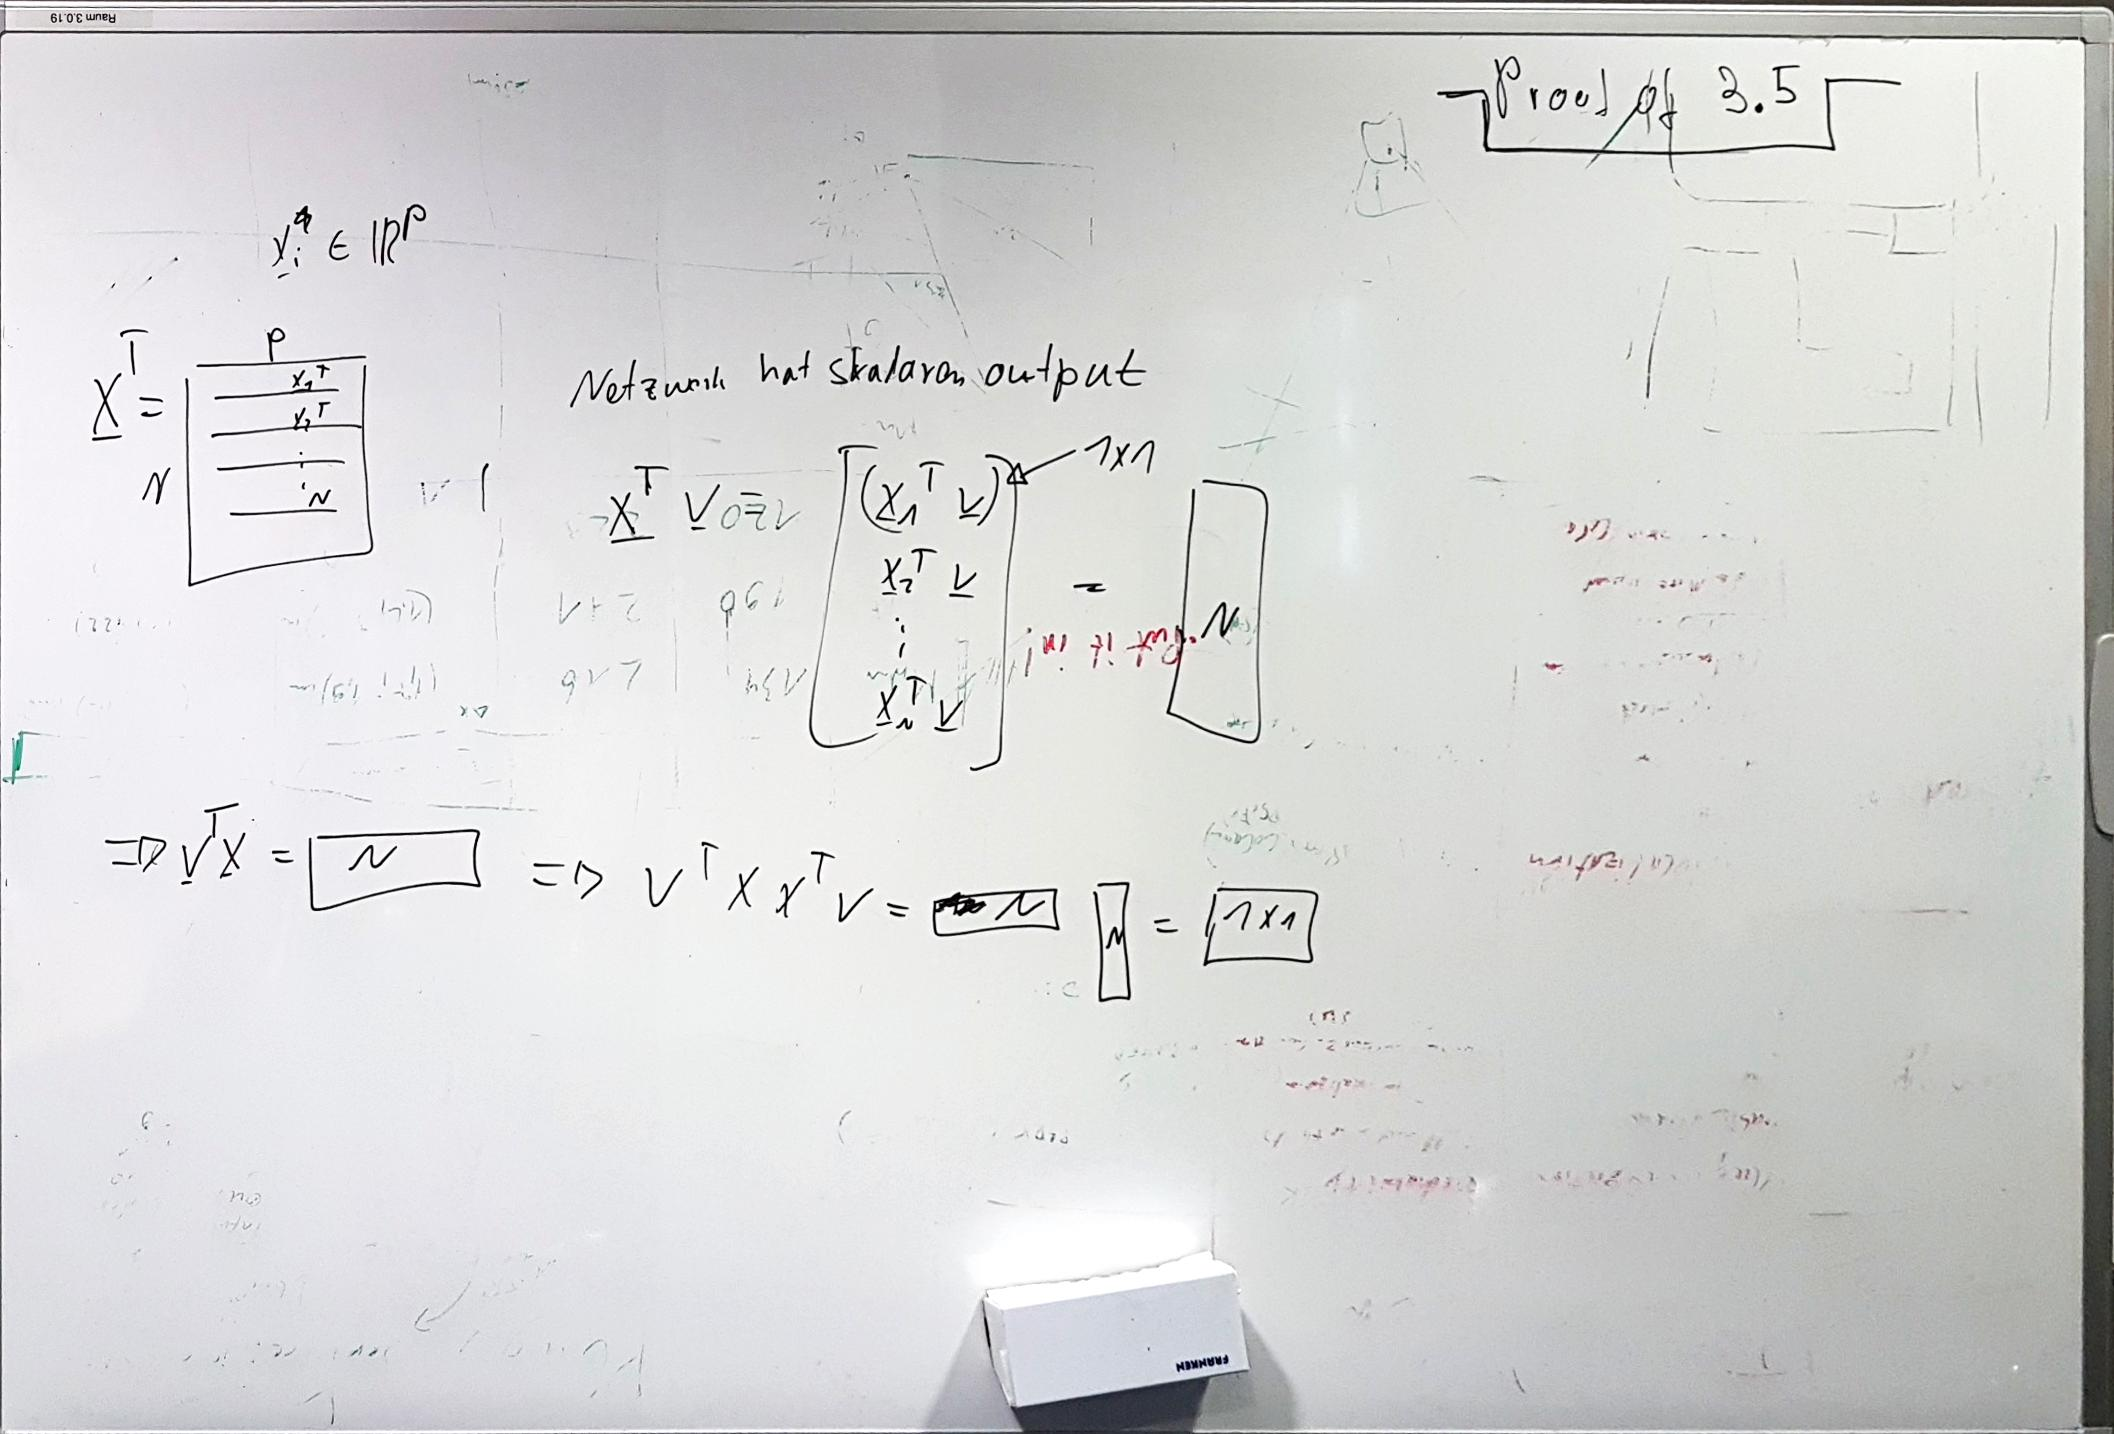
\includegraphics[width=\textwidth]{whiteboard_notes/10.jpg}
\end{figure}

\begin{figure}
	\centering
	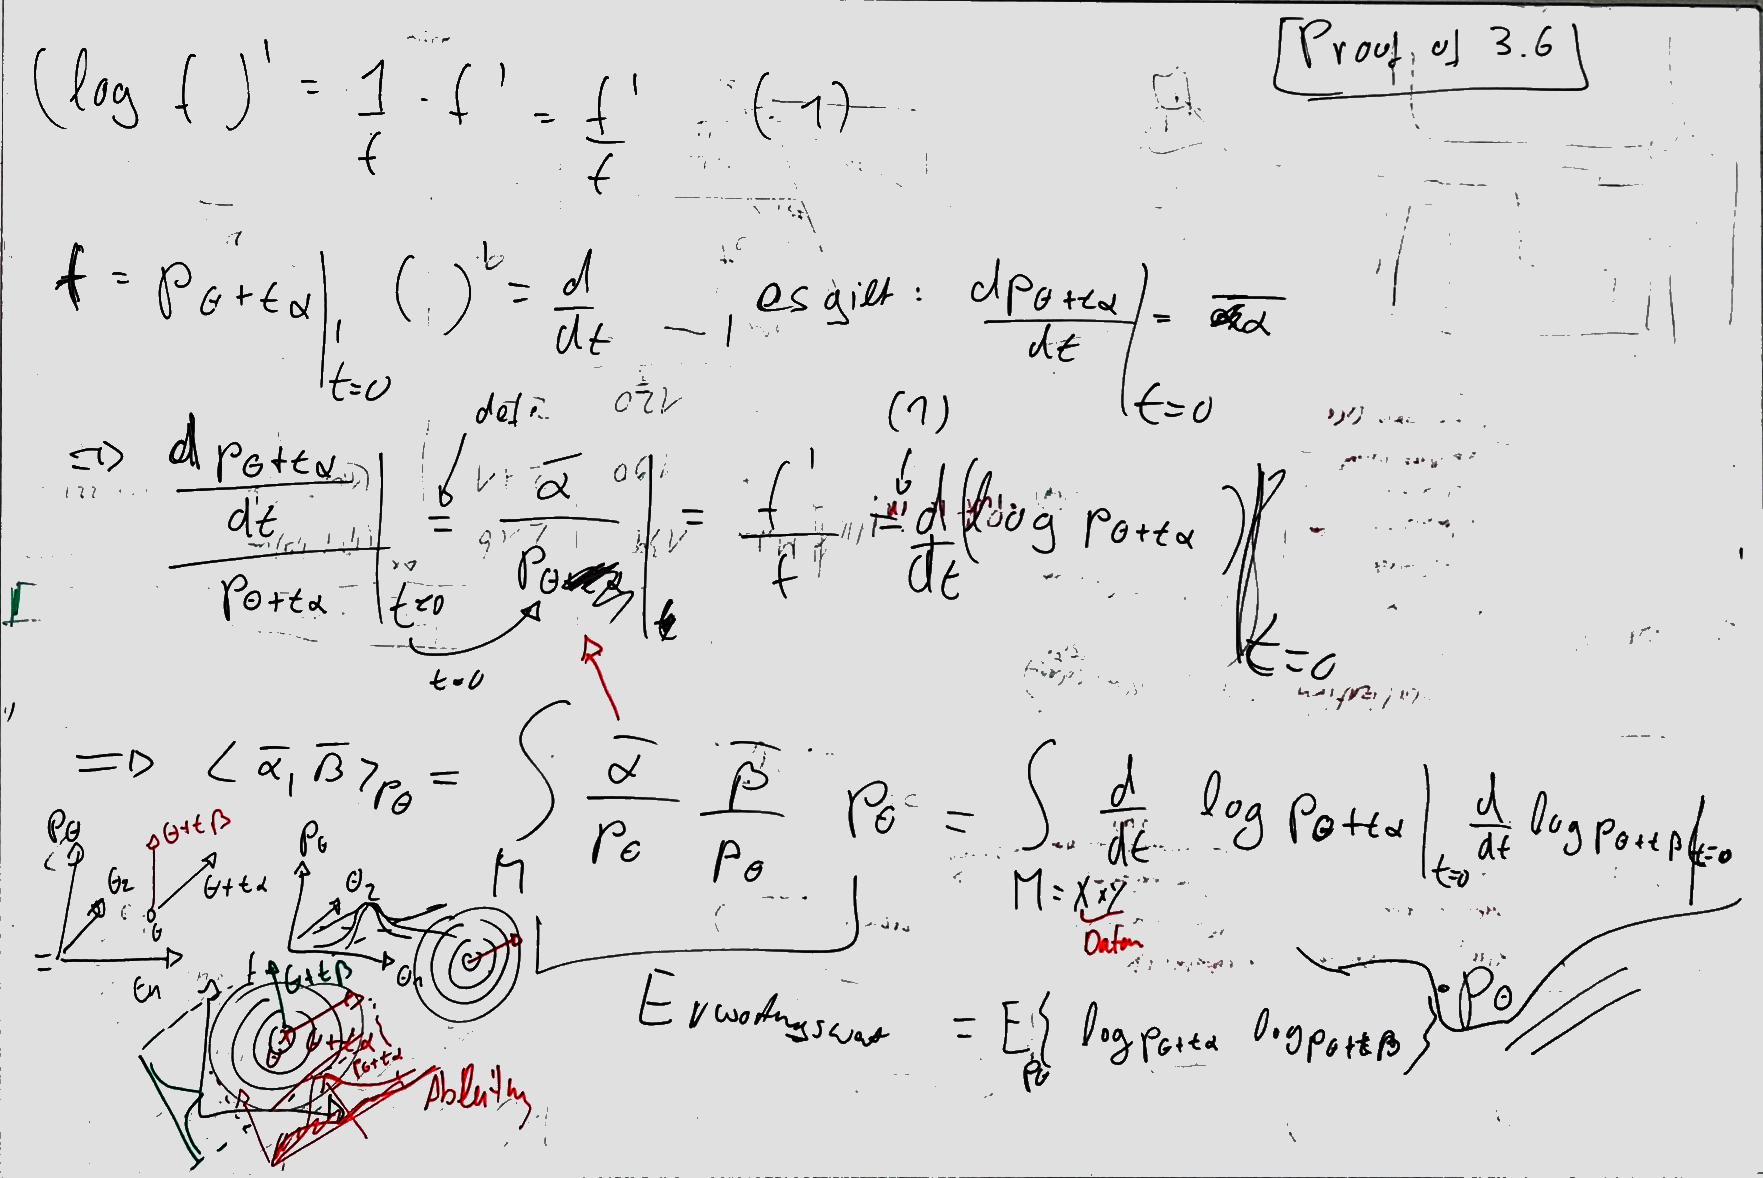
\includegraphics[width=\textwidth]{whiteboard_notes/11.jpg}
\end{figure}




\bibliographystyle{alpha}
\bibliography{sample}

\end{document}